\documentclass[12pt]{article}
\usepackage{ctex}
\usepackage{geometry}
\usepackage{hyperref}
\usepackage{listings}
\usepackage{xcolor}
\usepackage{amsmath}
\usepackage{graphicx}
\usepackage{subcaption}

\title{深度学习与神经网络第三次课程项目}
\author{王逸群 19307110397}
\date{2022.5}

\geometry{a4paper,left=2.5cm,right=2.5cm,top=2.5cm,bottom=2.5cm}

\hypersetup{
	colorlinks=true,
}

\definecolor{gray}{rgb}{0.99,0.99,0.99}

\lstdefinestyle{mystyle}{
	basicstyle=\footnotesize,
	backgroundcolor=\color{gray},
	numbers=left
}

\lstset{style=mystyle}

\begin{document}

\maketitle

\section{数据集介绍}

本项目使用MSCOCO(Microsoft Common Objects in Context)
数据集的子集,
并使用NOC(Novel Object Captioning)分割方法分割数据集。
数据集中的每张图片都附带5句人工标注的句子。
巴士、瓶子、沙发、微波炉、披萨、球拍、行李箱、斑马等8件物品
不出现在训练集中,但会出现在验证集和测试集中。

\section{模型学习}

\subsection{Deep Compositional Captioning}

Lisa Anne的DCC(Deep Compositional Captioning)模型
架构图如图\ref{fig:DCC}所示。
可以看到,模型由三个部分组成。 

\begin{figure}
	\centering
	\includegraphics[width=0.5\textwidth]{Papers/DCC.png}
	\caption{DCC模型架构图}
	\label{fig:DCC}
\end{figure}

首先,词汇分类器的主体是一个卷积神经网络。
其中,分类的目标概念是通过词性标注得到的
在图像文本对中频繁出现的形容词、动词和名词,
以及一些图像文本对以外的概念;
而分类器的输出是一个特征,
每个元素表示给定概念在图像中出现的概率。
具体操作时,词汇分类器先在ILSVRC(ImageNet Large Scale Visual Recognition Challenge)训练集上预训练,再进行精调。

接着,语言模型由词汇编码、长短期记忆网络、词汇预测层组成。
其中,生成的特征由词汇编码和长短期记忆网络的输出连接而成。

在词汇分类器和语言模型的基础上,图像说明模型由两者组合而成。
其中,词汇分类器的输出特征与语言模型的输出特征相互连接,
经过多模态单元即一个线性层和一个Softmax层后,
输出每一个单词是下一个单词的概率分布。

模型训练完毕后,还要进行知识迁移。

\subsection{Neural Baby Talk}

本项目使用Jiasen Lu的NBT(Neural Baby Talk)模型。
架构图如图\ref{fig:struct}所示。

\begin{figure}[h]
	\centering
	\includegraphics[width=0.5\textwidth]{Papers/NBT.png}
	\caption{NBT模型架构图}
	\label{fig:struct}
\end{figure}

该模型将单词分为两类进行处理,
一类是可视单词,基于特定的图片区域;
另一类是文本单词,是图像说明中的其它单词。
针对前者,还需要对其复数形式和细粒度形式进行判断。

\section{评价指标}

\subsection{F1}
\label{sec:F1}

将输出句子与标注句子中的单词分为四类:

\begin{table}[h]
	\centering
	\begin{tabular}{ccc}
		\hline
		名称 & 字母 & 含义 \\
		\hline
		真正例 & TP & 在输出句子和标注句子中都出现 \\
		假正例 & FP & 在输出句子中出现但在标注句子中不出现 \\
		假负例 & FN & 在输出句子中不出现但在标注句子中出现 \\
		真负例 & TP & 在输出句子和标注句子中都不出现 \\
		\hline
	\end{tabular}
	\caption{输出句子与标注句子中的四类单词}
\end{table}

定义精度、召回率、F1:
\begin{align*}
	P &= \frac{TP}{TP + FP} \\ 
	R &= \frac{TP}{TP + FN} \\ 
	F_1 &= \frac{2}{\frac{1}{P} + \frac{1}{R}} 
\end{align*}

\subsection{CIDEr}

CIDEr可以计算输出句子和一组标注句子的匹配程度。

首先,输出句子和标注句子的所有单词都被简化为词干,
进而输出句子和标注句子可以由一元至$N$元词汇表示。
默认情况下,$N=4$。

接着,
计算每个词元的TF-IDF权重。
具体而言,
记$I$表示待评判的输出句子集合。
对于第$i$句输出句子$c_i$,
有一组标注句子$S_i = \{s_{ij}\}$。
进而对于第$k$个词元,
记$h_k(c_i)$表示其在输出句子$c_i$中出现的次数,
$h_k(s_{ij})$表示其在标注句子$s_{ij}$中出现的次数,
于是TF-IDF权重为:
\begin{align*}
	g_k(c_i) &= \frac{h_k(c_i)}{\sum_l h_l(c_i)} \log (\frac{|I|}{\sum_p \min(1, h_k(c_p))}) \\
	g_k(s_{ij}) &= \frac{h_k(s_{ij})}{\sum_l h_l(s_{ij})} \log (\frac{|I|}{\sum_p \min(1, \sum_q h_k(s_{pq}))})
\end{align*}

在此基础上,再对于$n$元词汇,
计算输出句子和标注句子之间的TF-IDF的平均余弦相似度;
最后,将这些余弦相似度加权平均得到CIDEr;
\begin{align*}
	CIDEr_n(c_i, S_i) &= \frac{1}{|S_i|} \sum_j 
	\frac{g^n(c_i) \cdot g^n(s_{ij})}
	{||g^n(c_i)|| ||g^n(s_{ij})||} \\
	CIDEr(c_i, S_i) &= \sum_n w_n CIDEr_n(c_i, S_i)
\end{align*}

\subsection{METEOR}
\label{sec:METEOR}

对于给定的输出句子和标注句子,首先进行单词之间的对齐,
使得每个单词映射到另一个句子中的至多一个单词。
对齐包括若干个步骤,每个步骤包括两个阶段。

在第一阶段,若干外部模块根据不同的标准建立起所有可能的映射。
比如,\verb|exact|模块当两个单词完全相同时建立映射,
\verb|porter stem|模块当两个单词词干相同时建立映射,
\verb|WN synonymy|模块当两个单词是同义词时建立映射。
默认情况下,按顺序使用这三种模块。
在第二阶段,
第一阶段得到的所有可能的映射中的一个子集成为真正的映射,
该子集尽可能大,且尽可能产生较少的交叉。

得到单词之间的映射后,
使用与\ref{sec:F1}节相似的方法得到精度和召回率,
并计算:
\begin{equation*}
	F_{mean} = \frac{10}{\frac{1}{P} + \frac{9}{R}} 
\end{equation*}

由于以上仅进行了单词之间的对齐,
接下来需要再计算一个惩罚项,
体现词组甚至句子之间的对齐。
具体而言,
将输出句子中的单词聚合成尽可能少的块,
使得每一块中相邻的单词都映射到标注句子中相邻的单词。
这样一来,块越少,对齐的词组越长。进而得到惩罚项和MEREOR:
\begin{align*}
	Penalty &= \frac{1}{2} \times (\frac{\#chunks}{\#unigrams\_matched})^3 \\
	METEOR &= F_{mean} \times (1 − Penalty)
\end{align*}

\subsection{SPICE}

SPICE也可以计算输出句子和一组标注句子的匹配程度。

首先,对于每一句话,
计算其句法树,如图\ref{fig:SPICEsimple}上方所示;
并由句法树导出场景图,如图\ref{fig:SPICEsimple}右侧所示。
其中,实体、属性和联系分别被标注,图中显示为红色、绿色和蓝色。

\begin{figure}[h]
	\centering
	\includegraphics[width=0.75\textwidth]
	{Papers/SPICEsimple.png}
	\caption{句法树与场景图说明}
	\label{fig:SPICEsimple}
\end{figure}

具体而言,给定
实体集合$C$、
属性集合$A$、
联系集合$R$,
对于句子$c$,
记$O(c) \subseteq C$是$c$中出现的实体集合,
$K(c) \subseteq O(c) \times A$是$c$中出现的实体属性集合,
$E(c) \subseteq O(c) \times R \times O(c)$
是$c$中出现的实体联系集合,
则场景图为$G(c) = \langle O(c), E(c), K(c) \rangle$。

记输出句子$c$的场景图为$G(c)$,
每句标注句子$s_j$的场景图为$G(s_j)$。
将$G(s_j)$中同义实体的节点合并,
得到标注句子集合$S$的场景图$G(S)$,
如图\ref{fig:SPICEmultiple}所示。

\begin{figure}[h]
	\centering
	\includegraphics[width=0.75\textwidth]
	{Papers/SPICEmultiple.png}
	\caption{场景图合并说明}
	\label{fig:SPICEmultiple}
\end{figure}

最后,在场景图$G(c)$和$G(S)$的基础上,
使用\ref{sec:METEOR}中的对齐方法,
计算精度、召回率、F1,其中F1即为SPICE。

\section{实验过程中遇到的问题与解决}

\subsection{尝试安装Caffe}

\begin{itemize}
\item 运行\verb|transfer.sh|时,报错找不到模块\verb|caffe|,
通过\href{https://blog.csdn.net/jiyangsb/article/details/77724876}{网络}得知需要使用\verb|make _caffe| 命令编译C++程序文件;
编译时,又显示找不到C语言头文件\verb|Python.h|,通过\href{https://blog.csdn.net/slz0813/article/details/82961906#:~:text=%3Cbr%20%2F%3E%3Cbr%20%2F%3E%E5%87%BA%E7%8E%B0%20No%20such%20file%20or%20directory,%E7%9A%84%E9%94%99%E8%AF%AF%EF%BC%8C%E6%9C%89%E4%B8%A4%E7%A7%8D%E6%83%85%E5%86%B5%EF%BC%8C%E4%B8%80%E7%A7%8D%E6%98%AF%E7%9C%9F%E7%9A%84%E6%B2%A1%E6%9C%89%20Python.h%E8%BF%99%E4%B8%AA%E6%96%87%E4%BB%B6%EF%BC%8C%E4%B8%80%E7%A7%8D%E6%98%AF%20Python%20%E7%9A%84%E7%89%88%E6%9C%AC%E4%B8%8D%E5%AF%B9%EF%BC%8C%3Cbr%20%2F%3E%E5%8F%AF%E4%BB%A5%E8%BF%9B%E5%85%A5%2Fusr%2Finclude%2F%E6%96%87%E4%BB%B6%E5%A4%B9%E4%B8%8B%E7%9A%84%20Python%202.x%E6%96%87%E4%BB%B6%E5%A4%B9%E9%87%8C%E6%9F%A5%E6%89%BE%E6%98%AF%E5%90%A6%E6%9C%89%20Python.h%E8%BF%99%E4%B8%AA%E6%96%87%E4%BB%B6%E3%80%82}{网络}得知需要安装对应的文件,操作后并未解决问题;
再通过\href{https://blog.csdn.net/Hello_Orange/article/details/6184420}{网络}得知C语言包含头文件的搜索路径,确保以下路径中都有\verb|Python.h|:
\begin{lstlisting}
/usr/include/
/usr/local/include/
/usr/local/miniconda3/include/
/usr/local/miniconda3/envs/DCC/include/
\end{lstlisting}
仍然没有解决问题;
最后通过\href{https://www.cnblogs.com/xiel/p/3613919.html}{网络}得知,使用\verb|gcc|命令编译C++程序文件时,可以通过参数\verb|-I|指定头文件的搜索路径,解决问题。
% gcc utils/tools/caffe/_caffe.cpp -I /usr/local/miniconda3/envs/DCC/include/python2.7
\item 继续编译C++程序文件,又显示找不到C语言头文件\verb|numpy/arrayobject.h|,与上面的问题相似,通过\href{https://blog.csdn.net/wuzuyu365/article/details/52430657}{网络}得知需要运行\verb|sudo apt-get install python-numpy|安装对应的文件,解决问题。
\item 继续编译C++程序文件,又显示找不到C语言头文件\verb|caffe/proto/caffe.pb.h|,通过\href{https://blog.csdn.net/ycz28/article/details/78920140}{网络}得知需要使用\verb|protoc|从\verb|src/caffe/proto/caffe.proto|生成\verb|caffe.pb.h| 和 \verb|caffe.pb.cc|,解决问题。
至此,C++程序文件成功编译。
\item 继续运行\verb|transfer.sh|时,依然报错找不到模块\verb|caffe|,通过\href{https://blog.csdn.net/silverdemon/article/details/77752873}{网络}得到一种解决方法,修改\verb|PYTHONPATH|,操作后并未解决问题。
\item 在室友的指导下,转而使用\verb|Makefile|编译,即使用\verb|make|命令;
编译时,报错无法创建链接,通过\href{https://blog.csdn.net/guozhongwei1/article/details/82834848}{网络}推测与服务器远程主页有关,于是将文件夹移动至服务器根目录,该报错信息不再出现。
\item 继续使用\verb|make|命令编译,显示找不到C语言头文件\verb|hdf5.h|,通过\href{https://blog.csdn.net/uuuuur/article/details/109367417}{网络}指示先安装对应的文件,操作后并未解决问题,使用\verb|find|命令查找路径,并在\verb|Makefile.config|文件中修改\verb|INCLUDE_DIRS := $(PYTHON_INCLUDE) /usr/local/include|路径,该报错信息不再出现。
% cp /remote-home/wangyiqun/Project03/DCC/caffe/Makefile.config /root/caffe
\item 
继续使用\verb|make|命令编译,显示找不到C语言头文件\verb|lmdb.h|,通过\href{https://blog.csdn.net/sdlypyzq/article/details/85236736}{网络}指示安装对应的文件,与上面的问题相似,使用\verb|find|命令查找路径,并在\verb|Makefile.config|文件中修改\verb|INCLUDE_DIRS := $(PYTHON_INCLUDE) /usr/local/include|路径,该报错信息不再出现。
\item 继续使用\verb|make|命令编译,显示不支持GPU架构,通过\href{https://www.jianshu.com/p/cc7a405322e3}{网络}指示在\verb|Makefile.config| 文件中修改\verb|CUDA_ARCH|,该报错信息不再出现。
\item 继续使用\verb|make|命令编译,显示如下报错信息:
\begin{lstlisting}
/usr/bin/ld: cannot find -lhdf5_hl
/usr/bin/ld: cannot find -lhdf5
/usr/bin/ld: cannot find -lleveldb
/usr/bin/ld: cannot find -lsnappy
\end{lstlisting}
针对前两项,通过\href{https://796t.com/content/1548083182.html}{网络}指示在\verb|Makefile|文件中修改\verb|LIBRARIES|变量;
针对后两项,通过\href{https://www.cnblogs.com/z-books/p/4171195.html}{网络}指示,与最早的问题类似,安装对应的文件,该报错信息不再出现。
\item 继续使用\verb|make|命令编译,显示存在未定义的引用,通过\href{https://blog.csdn.net/weixin_41770169/article/details/90413895}{网络}指示在\verb|Makefile|文件中修改\verb|LIBRARIES|变量,该报错信息不再出现。至此,成功使用\verb|make|命令编译。
\item 继续运行\verb|transfer.sh|时,依然报错找不到模块\verb|caffe|,通过\href{https://blog.csdn.net/cui841923894/article/details/81639290}{网络}指示,
运行命令\verb|make pycaffe|,
并修改\verb|PYTHONPATH|,
该报错信息不再出现。
\item 继续运行\verb|transfer.sh|时,又报错找不到模块\verb|skimage.io|,通过\href{https://blog.csdn.net/u010205128/article/details/80995358}{网络}得知需要运行 \verb|sudo apt-get install python-skimage|安装对应的文件,操作后并未解决问题;再通过\href{https://www.cnblogs.com/zhuiluoyu/p/5181098.html}{网络}得知可以使用\verb|dpkg|命令获取\verb|skimage|的安装路径;根据之前的经验,修改\verb|PYTHONPATH|,该报错信息不再出现。
\end{itemize}

\subsection{尝试运行NBT代码}

\begin{itemize}
\item 运行\verb|docker|命令时,显示找不到\verb|docker|命令,通过\href{https://cloud.tencent.com/developer/article/1605163}{网络}指示操作,显示找不到\verb|yum|命令;再通过\href{https://www.jianshu.com/p/d4a32d420525}{网络}指示安装\verb|yum|命令,报错找不到模块\verb|rpm|;再通过\href{https://blog.csdn.net/xTand/article/details/105710793}{网络}指示安装\verb|yum|命令,操作后并未解决问题;再通过\href{https://blog.csdn.net/weixin_44037416/article/details/102608113}{网络}指示安装\verb|yum|命令,成功;通过\href{https://www.linuxidc.com/Linux/2020-01/162075.htm#:~:text=Linux%20CentOS%207%20%E9%9D%9Eroot%E7%94%A8%E6%88%B7%E5%AE%89%E8%A3%85%E6%BA%90%E7%A0%81%E7%89%88Docker%201%201.%E6%9F%A5%E7%9C%8B%E5%BD%93%E5%89%8D%E4%B8%BB%E6%9C%BA%E6%98%AF%E5%90%A6%E6%9C%89docker%E7%BB%84%202%203.%E6%8A%8A%E5%BD%93%E5%89%8D%E7%94%A8%E6%88%B7%E5%8A%A0%E5%85%A5%E5%88%B0docker%E7%BB%84,%2Fusr%2Fb%20...%207%206.%E5%B0%86docker%E6%B3%A8%E5%86%8C%E4%B8%BAservice%E6%9C%8D%E5%8A%A1%208%207.%E6%B7%BB%E5%8A%A0%E6%89%A7%E8%A1%8C%E6%9D%83%E9%99%90%E5%B9%B6%E9%87%8D%E6%96%B0%E5%8A%A0%E8%BD%BD%E9%85%8D%E7%BD%AE%E6%96%87%E4%BB%B6%209%209.%E5%90%AF%E5%8A%A8docker}{网络}指示安装\verb|docker|命令,成功,但是不能启动\verb|docker|。
\item 使用\verb|pip|命令安装\verb|pycocotools|模块时报错,通过\href{https://blog.csdn.net/weixin_42840933/article/details/85308265}{网络}指示,成功安装;使用\verb|pip|命令安装\verb|stanfordcorenlp|模块时报错,通过\href{https://blog.csdn.net/maxMikexu/article/details/105459045}{网络}指示,用相似的方法成功安装。
\item 运行\verb|main.py|程序时,报错\verb|torch.utils.ffi|模块已弃用,在室友的指导下,通过\href{https://blog.csdn.net/qq_45750017/article/details/118997481}{网络}指示,更换\verb|torch|的版本为\verb|0.4.0|,\verb|torchvision|的版本为\verb|0.2.2|,\verb|torchtext|的版本为\verb|0.2.3|,\verb|tensorflow|的版本为\verb|1.15.0|,该报错信息不再出现。
\item 运行\verb|main.py|程序时,使用\verb|torchtext.vocab.GloVe|下载\verb|glove.6B.zip|,报错拒绝连接,通过\href{https://blog.csdn.net/weixin_56915683/article/details/118000821}{网络}指示,手动下载\verb|glove.6B.zip|,并移动到\verb|.vector_cache|文件夹。
% \item 运行\verb|main.py|程序时,报错\verb|tensorboard|找不到相应的属性,通过\href{https://blog.csdn.net/u010556156/article/details/103320010}{网络}得知存在版本问题,将\verb|tf.summary.FileWriter|改为\verb|tf.summary.create_file_writer|,该报错信息不再出现;又报错\verb|tensorboard|找不到属性\verb|Summary|,通过\href{https://blog.csdn.net/chenying212chenkun/article/details/105032282}{网络}得知存在版本问题,将\verb|tf.Summary|改为\verb|tf.compat.v1.Summary|,该报错信息不再出现。
\item 运行\verb|main.py|程序时,读取\verb|h5|文件会频繁且随机地报错,相同的程序在室友的服务器上可以正常运行,因此之后在室友的帮助下在室友的服务器上完成程序运行。
\end{itemize}

\section{数据预处理}

\begin{itemize}
\item 使用Karpathy对MSCOCO数据集的预处理:将所有单词转化为小写,丢弃非字母数字的字符,保留在训练集中至少出现5次的单词。
% /data/dataset_coco.json
\item 使用Faster-RCNN对MSCOCO数据集进行目标检测。
% /data/coco/coco_detection.h5
\end{itemize}

\section{模型预训练}

\begin{itemize}
\item 以ResNet-101为初始架构,在ImageNet上预训练模型。
% /data/imagenet_weights/resnet101.pth
\end{itemize}

\section{超参数设置}

\begin{itemize}
\item beam size:训练时为1,测试时为3;
\item 梯度截断:0.1;
\item 学习率:初始值为0.0005,之后每3个回合下降为0.8倍;
\item 权重衰减:无;
\item 优化器:参数为0.9和0.999的Adam优化器;
\item 回合数:30;
\item 批量大小:20。
\end{itemize}

\section{实验结果}

实验结果如图\ref{fig:result}和表\ref{tab:result}所示。

\begin{figure}[h]
	\centering
	\begin{subfigure}{0.49\textwidth}
		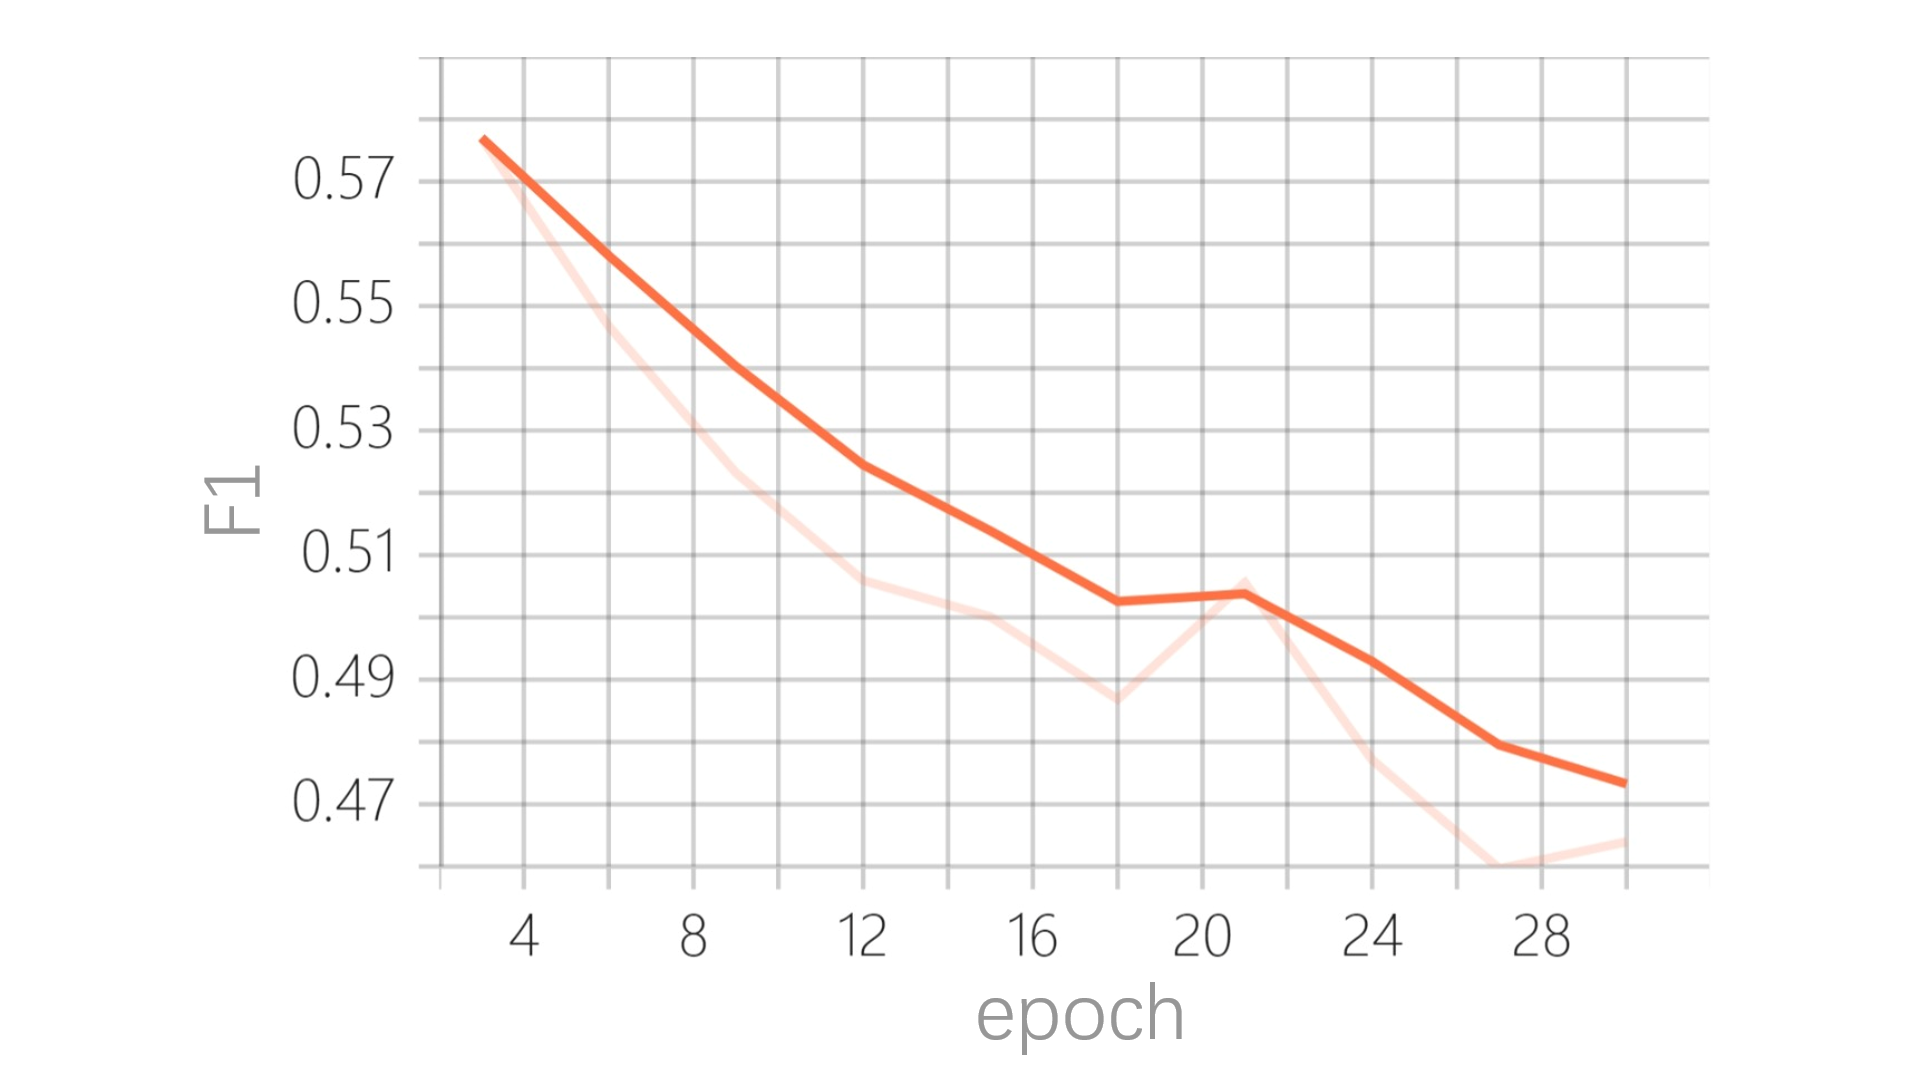
\includegraphics[width=\linewidth]{Plot/F1.png}
	\end{subfigure}
	\begin{subfigure}{0.49\textwidth}
		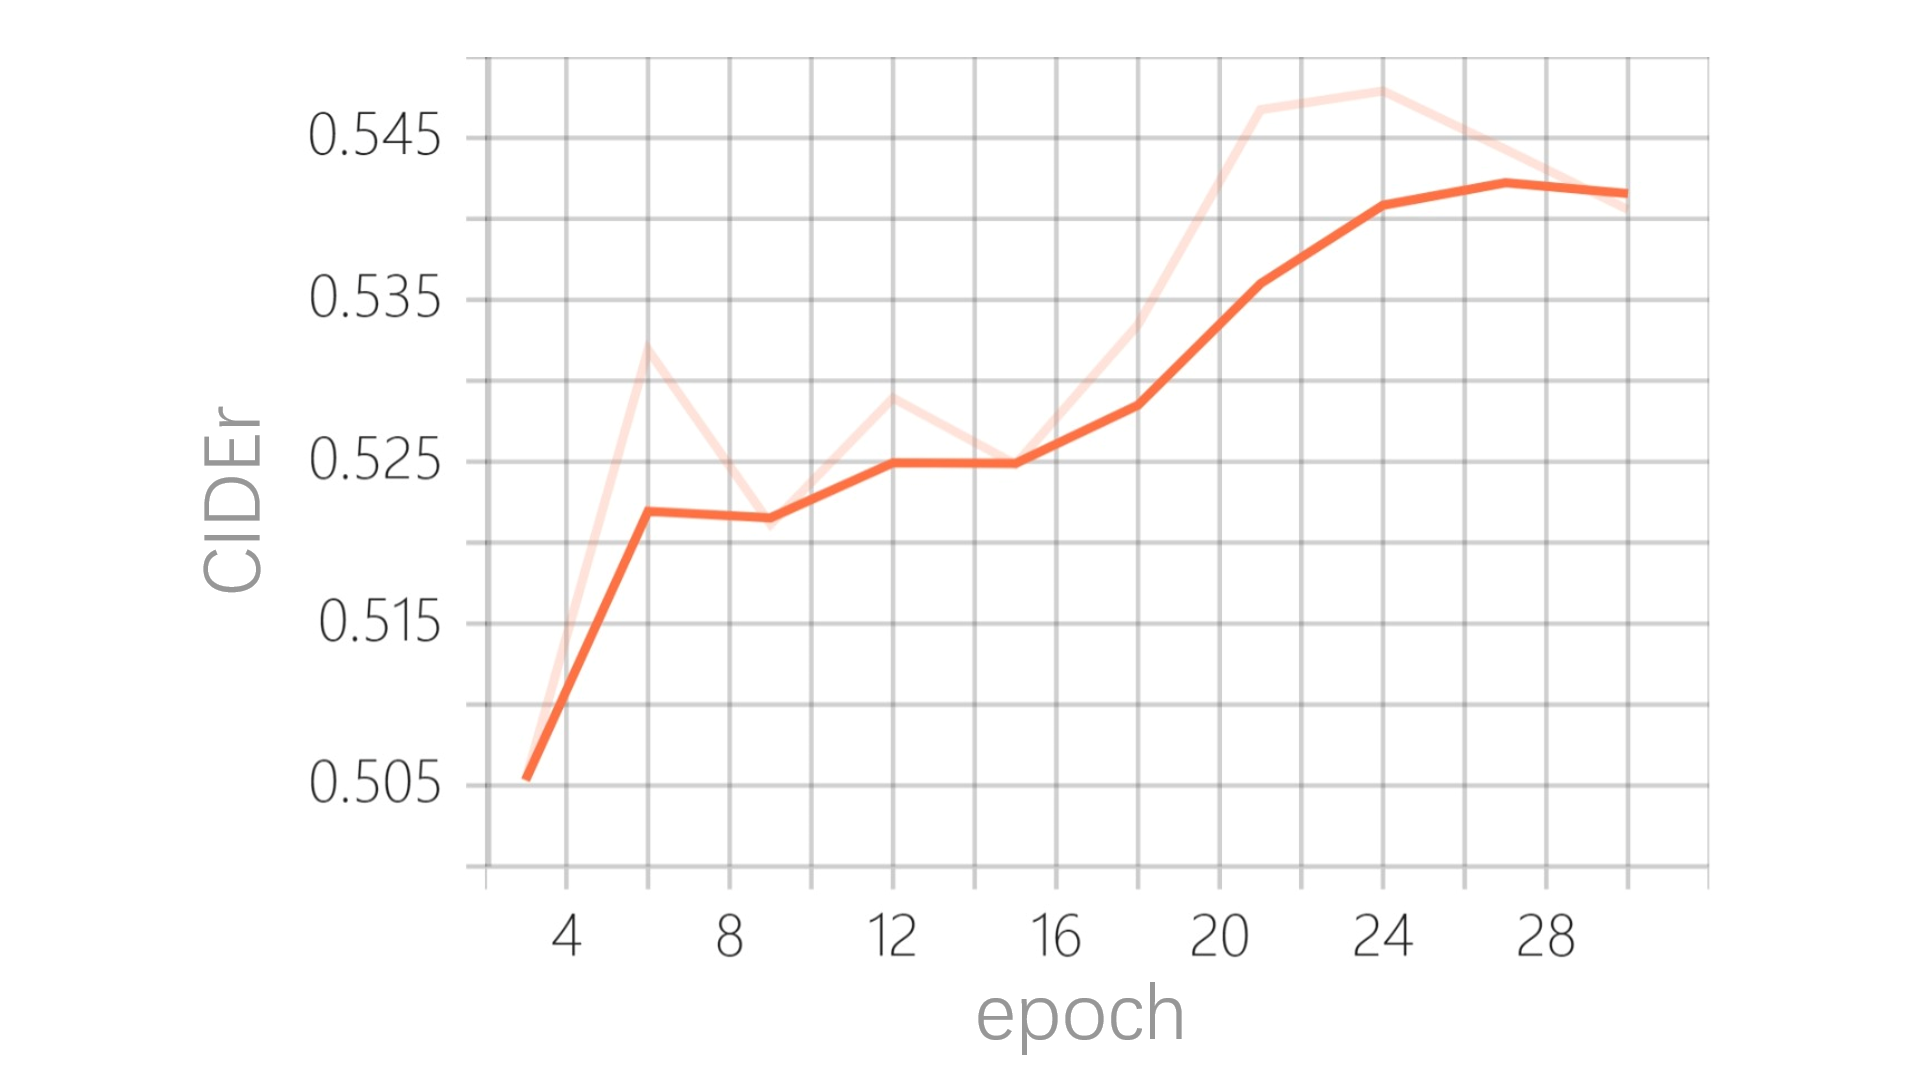
\includegraphics[width=\linewidth]{Plot/CIDEr.png}
	\end{subfigure}
	\begin{subfigure}{0.49\textwidth}
		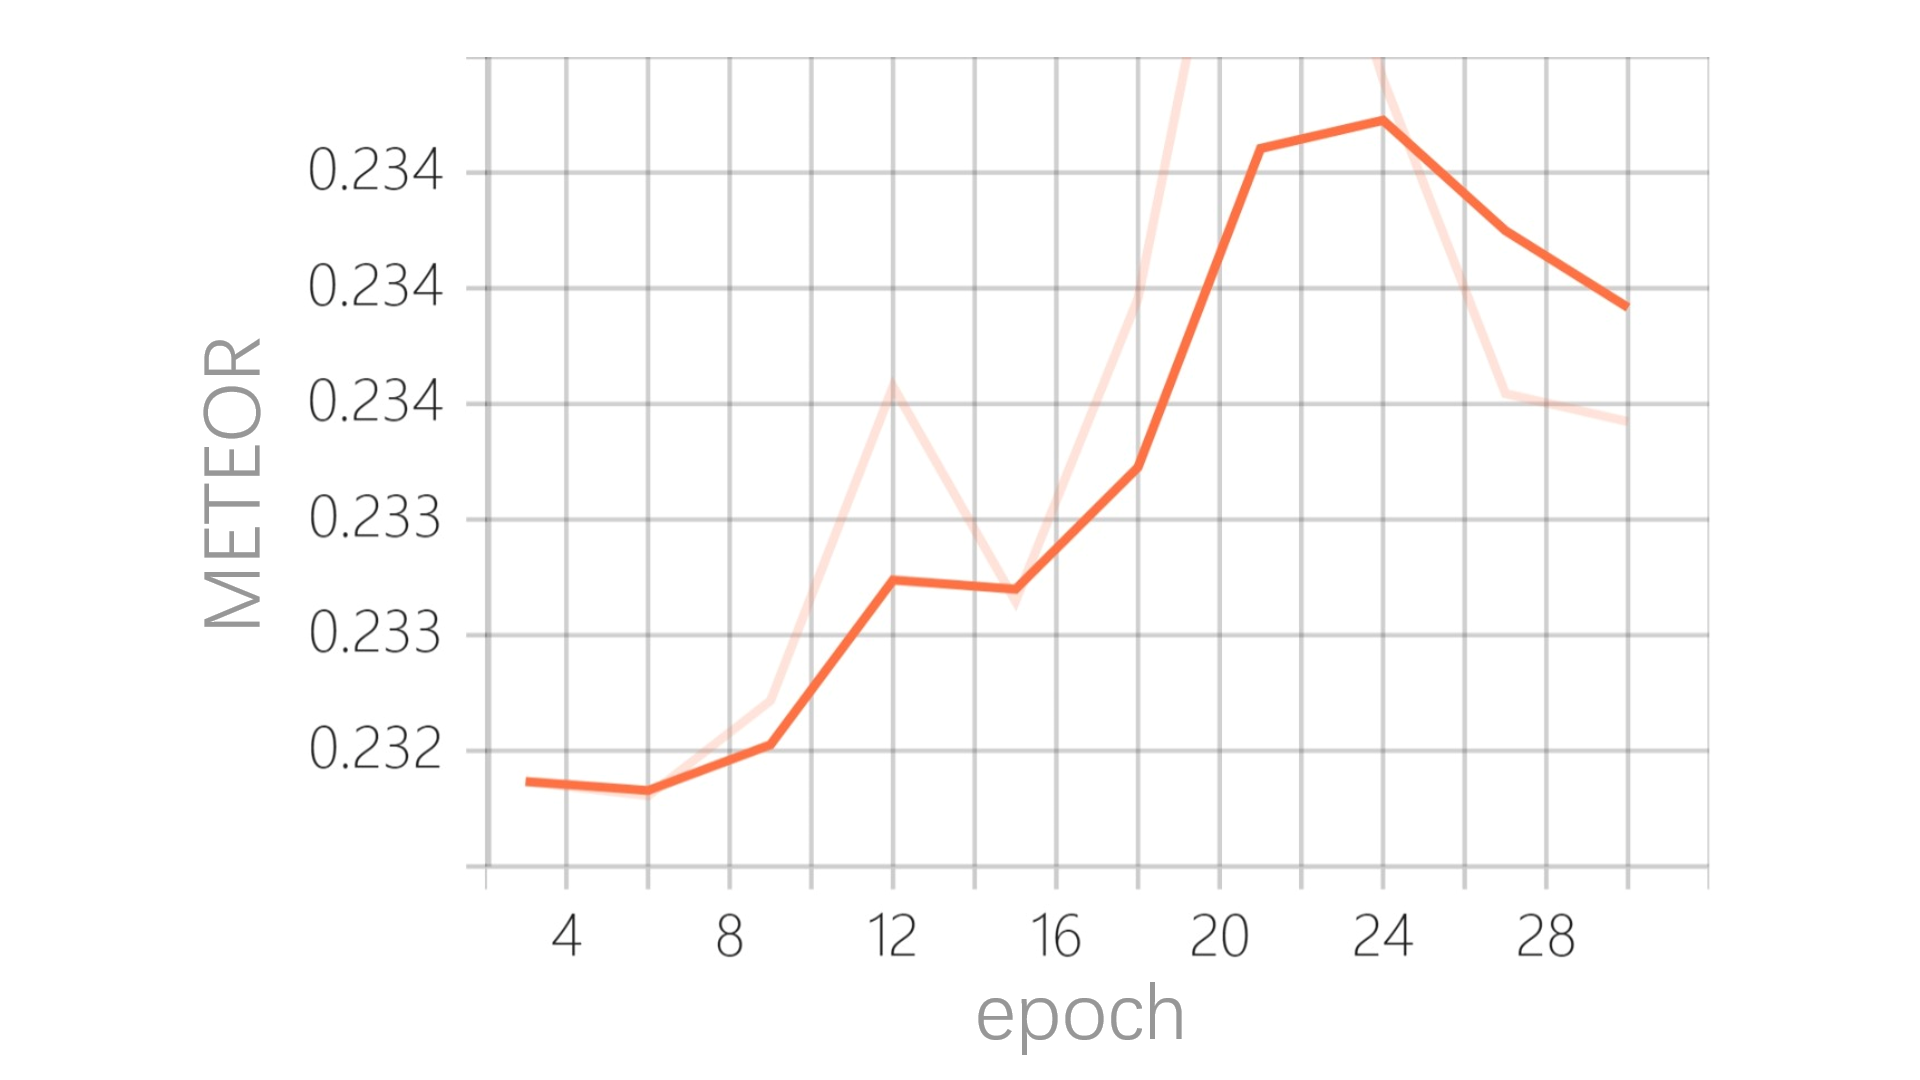
\includegraphics[width=\linewidth]{Plot/METEOR.png}
	\end{subfigure}
	\begin{subfigure}{0.49\textwidth}
		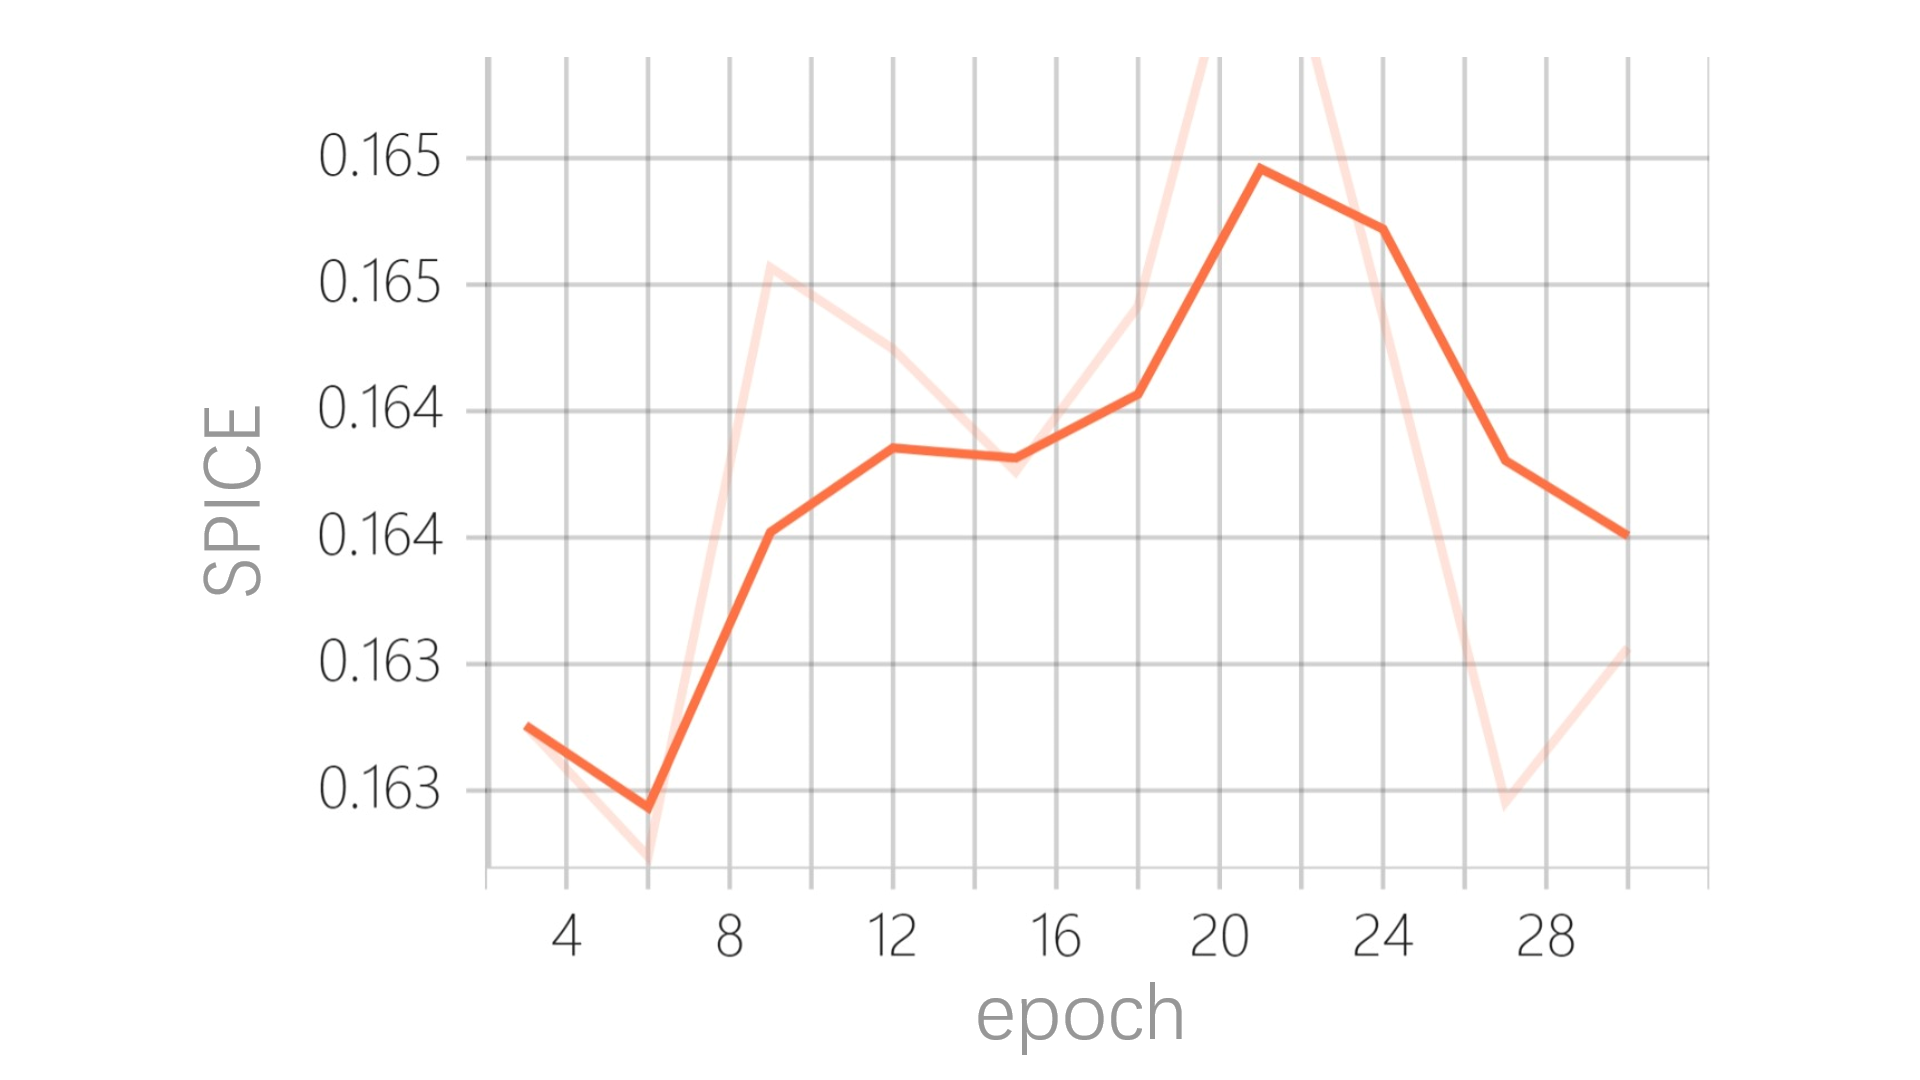
\includegraphics[width=\linewidth]{Plot/SPICE.png}
	\end{subfigure}
	\caption{实验结果}
	\label{fig:result}
\end{figure}

\begin{table}[h]
	\centering
	\begin{tabular}{|l|cccccccc|c|} 
		\hline
		& 巴士 & 瓶子 & 沙发 & 微波炉
		& 披萨 & 球拍 & 行李箱 & 斑马 & 平均 \\
		\hline
		F1 & 0.683 & 0.075 & 0.300 & 0.584
		& 0.347 & 0.146 & 0.470 & 0.888 & 0.437 \\
		CIDEr & 0.523 & 0.804 & 0.685 & 0.543 
		& 0.510 & 0.334 & 0.626 & 0.426 & 0.556 \\
		METEOR & 0.223 & 0.222 & 0.259 & 0.244 
		& 0.209 & 0.242 & 0.213 & 0.231 & 0.231 \\
		SPICE & 0.174 & 0.161 & 0.185 & 0.161 
		& 0.150 & 0.166 & 0.146 & 0.172 & 0.164 \\
		\hline
	\end{tabular}
	\caption{实验结果}
	\label{tab:result}
\end{table}

可以看到,
随着训练过程的推进,
CIDEr、METEOR、SPICE等评价指标都有上升的趋势,
而F1有下降的趋势。
前者能够比较好地评价句子的语义信息,
较有参考价值;
而后者则相反,
参考价值较低。

\end{document}